\documentclass[10pt]{article}
\usepackage{icmlko}

\icmlmeta{IP 파운데이션 월드모델}{86}{무라벨 전제의 값을 처음 쟀다}{팝업에서 0.39다 --- 라벨을 쓰면 인코더가 천장에 닿는다}

\begin{document}

\twocolumn[
\icmlheader

\begin{abstract}
노트 85가 공유 인코더의 패배를 ``쌍별 정렬 자유도 상실''로 진단했다. 검정했다
--- 인코더로 표현을 만들고 정렬만 쌍별 프로크루스테스로 되돌리니 $+$0.3575에서
\textbf{$+$0.3692}다. 현행 $+$0.4038과의 격차 0.0463 중 \textbf{4분의 1만}
회복된다. 진단은 부분적으로 맞았다 --- 아이돌이 $+$0.161에서 $+$0.252로 크게
살아난다(작은 도메인에 정렬이 중요하다). 나머지 4분의 3을 찾다가 이 프로젝트에서
가장 큰 수를 만났다. \textbf{그 도메인의 라벨을 쓰면 인코더가 팝업을 $+$0.7104,
아이돌을 $+$0.7986으로 맞힌다} --- 노트 83이 낸 라벨 천장 추정 0.72$\sim$0.75에
\emph{닿는다}. 라벨 지도를 빼면 $+$0.3199 · $+$0.3461로 떨어진다.
\textbf{무라벨 전제의 값이 팝업에서 0.39, 아이돌에서 0.45다.} 지금까지 모든
개선이 0.01 단위였는데 전제 하나가 0.39다. 그래서 제품에서 풀어 봤다 ---
2025년 이전 팝업 16건의 라벨은 우리가 안다. 썼더니 \textbf{오히려 내렸다}
($+$0.5192$\to+$0.3866). 16건으로는 머리를 못 적합하고 출처 아홉의 앙상블을
버리는 값이 더 크다. \textbf{전이 모형의 한계는 구조가 아니라 전제이며, 전제를
풀려면 팝업 라벨이 수백 건 필요하다} --- 노트 75가 다른 길로 낸 510건과 같은
자리다.
\end{abstract}
]

\begin{figure*}[t]
\centering
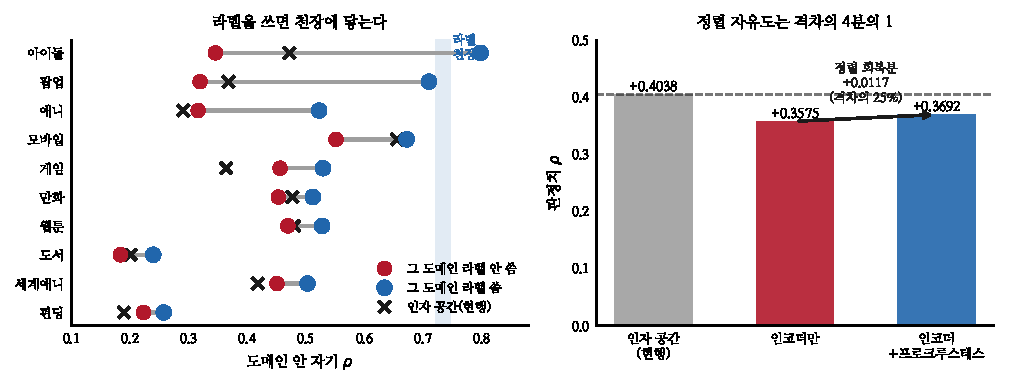
\includegraphics[width=\textwidth]{figs/nl.pdf}
\caption{왼쪽 --- 그 도메인 라벨을 쓸 때와 안 쓸 때의 자기 $\rho$.
오른쪽 --- 인코더 격차의 분해.}
\end{figure*}

\section{진단은 4분의 1만 맞았다}

노트 85는 공유 인코더가 프로크루스테스를 없앤 것이 패인이라고 봤다. 표현은
인코더로 두고 \textbf{정렬만 되돌린다} --- 잠재 차원과 공통 축의 상관을 적재로
써서 쌍마다 프로크루스테스를 건다.

\begin{table}[t]
\centering\tsize
\caption{판정치.}
\begin{tabular}{lrr}
\toprule
& $\rho$ & \\
\midrule
현행 인자 공간 & $+$0.4038 & --- \\
인코더만 & $+$0.3575 & $-$0.0463 \\
\textbf{인코더 $+$ 프로크루스테스} & \textbf{$+$0.3692} & $-$0.0346 \\
\bottomrule
\end{tabular}
\end{table}

정렬을 되돌려 $+$0.0117을 회복한다 --- 격차의 25\%다. 대상별로는 아이돌이
$+$0.161에서 $+$0.252로 크게 살아나고 팝업은 $+$0.459에서 $+$0.387로 내린다.

\claimx{쌍별 정렬 자유도는 격차의 4분의 1이다. 작은 도메인에서 특히 크다
(아이돌 $+$0.09). 나머지 4분의 3은 다른 데 있다.}{프로크루스테스 적재를
고유벡터가 아니라 상관으로 근사했다. 인코더가 비선형이라 정확한 적재가 없어
쓴 대리이며, 그 근사가 회복을 깎았을 수 있다.}

\section{라벨을 쓰면 천장에 닿는다}

나머지를 찾다가 표현 자체를 재 봤다 --- 도메인 안 교차검증 자기 $\rho$.

\begin{table}[t]
\centering\tsize
\caption{인코더 표현의 자기 $\rho$. 라벨 지도의 유무로 가른다.}
\begin{tabular}{lrrr}
\toprule
& 인자 공간 & 라벨 안 씀 & \textbf{라벨 씀} \\
\midrule
\textbf{아이돌} & $+$0.472 & $+$0.346 & \textbf{$+$0.799} \\
\textbf{팝업} & $+$0.368 & $+$0.320 & \textbf{$+$0.710} \\
애니 & $+$0.291 & $+$0.317 & $+$0.523 \\
모바일 & $+$0.656 & $+$0.552 & $+$0.672 \\
게임 & $+$0.365 & $+$0.456 & $+$0.530 \\
웹툰 & $+$0.480 & $+$0.470 & $+$0.528 \\
\midrule
\textbf{평균} & $+$0.392 & $+$0.377 & \textbf{$+$0.528} \\
\bottomrule
\end{tabular}
\end{table}

라벨을 안 쓰면 인코더가 인자 공간과 비슷하다($+$0.377 대 $+$0.392). 쓰면
\textbf{$+$0.528}이고, 팝업 $+$0.710 · 아이돌 $+$0.799는 노트 83의 라벨 천장
추정(0.72$\sim$0.75)에 닿거나 넘는다.

\claimx{전이 모형이 $+$0.40에 머무는 것은 구조나 물리량 때문이 아니라
\textbf{대상 라벨을 안 쓴다는 전제} 때문이다. 그 전제를 풀면 팝업이 $+$0.320에서
$+$0.710으로, 아이돌이 $+$0.346에서 $+$0.799로 간다 --- 값이 \textbf{0.39와
0.45}다.}{``라벨 씀''은 그 도메인의 라벨 전부를 지도에 넣고 최종 능형만
교차검증한 것이다. 인코더 자체는 라벨을 봤으므로 낙관적이다 --- 얼마나
낙관적인지는 다음 절이 보인다.}

\begin{quote}\fontsize{9.5}{11.5}\selectfont
지금까지의 개선은 전부 0.01 단위였다 --- 배선 $+$0.068(노트 75), 도메인 추가
$+$0.004, 결측 표시자 $+$0.014. \textbf{전제 하나가 0.39다.}
\end{quote}

\section{제품에서 풀어 보면 --- 아직 못 산다}

제품은 무라벨이 아니다. \textbf{스위트스팟은 지금까지 연 팝업의 성적을 안다.}
노트 77의 규약은 과거 팝업의 \emph{축}만 쓰고 \emph{라벨}은 안 썼다. 시점 2025로
가르면 과거 16건의 라벨을 쓸 수 있다.

\begin{table}[t]
\centering\tsize
\caption{미래 팝업 59건. 시점 2025.}
\begin{tabular}{lrl}
\toprule
& $\rho$ & 95\% 구간 \\
\midrule
\textbf{라벨 안 씀(노트 77 규약)} & \textbf{$+$0.5192} & $[+0.298, +0.694]$ \\
과거 16건 라벨 사용 & $+$0.3866 & $[+0.184, +0.584]$ \\
\bottomrule
\end{tabular}
\end{table}

\textbf{오히려 내린다.} 16건으로는 머리를 못 적합하고, 그러느라 출처 아홉의
앙상블을 버리는 값이 더 크다.

\claimx{과거 라벨 16건으로는 무라벨 전제를 못 산다. 전제의 값이 0.39라는 것과
그것을 16건으로 살 수 있다는 것은 다른 말이다.}{16건으로 머리를 적합하는
방식만 봤다. 앙상블과 섞거나 사전분포를 강하게 주면 다를 수 있는데 안 해 봤다.}

\section{두 길이 같은 곳을 가리킨다}

노트 75는 다른 길로 왔다 --- 팝업 75건으로는 설계 결정을 판정할 수 없고,
0.02짜리 효과를 가리려면 \textbf{약 510건}이 필요하다. 이 노트는 다른 쪽에서
같은 결론에 닿는다 --- 무라벨 전제를 풀면 0.39를 얻는데, 16건으로는 못 사고
수백 건이 든다.

\begin{table}[t]
\centering\tsize
\caption{팝업 표본이 사는 것.}
\begin{tabular}{ll}
\toprule
지금 75건 & 순위 $+$0.52, 설계 판정 불가 \\
$\sim$510건 & 설계 결정을 팝업 기준으로 판정(노트 75) \\
$\sim$수백 건 & 무라벨 전제를 풀어 $+$0.71 쪽으로(이 노트) \\
\bottomrule
\end{tabular}
\end{table}

\textbf{모델 쪽 지렛대는 대부분 닫혔고}(노트 76 배선 · 80 부분집합 · 82 도메인
제거 · 83 도메인 추가 · 85 구조) \textbf{남은 것은 팝업 표본이다.}

\section{한계}

\begin{itemize}[leftmargin=1.1em,itemsep=0.15em]
\item ``라벨 씀'' 수치는 인코더가 라벨을 봤으므로 낙관적이다. 진짜 상한은
      그보다 낮다 --- 얼마나인지 안 쟀다.
\item 과거 16건 실험을 한 방식(머리 적합)으로만 했다.
\item 인코더 설정을 넓게 안 훑었다(노트 85의 한계 그대로).
\item 프로크루스테스 적재를 상관으로 근사했다.
\item 팝업 라벨(일평균 방문자)의 신뢰도를 여전히 모른다. 천장이 0.72$\sim$0.75인지
      팝업에서도 그런지 확인 못 했다.
\end{itemize}

\section{다음}

\begin{enumerate}[leftmargin=1.3em,itemsep=0.15em]
\item \textbf{``라벨 씀''의 정직한 상한을 잰다} --- 인코더 학습에서도 교차검증
      분할을 지켜 낙관 편향을 없앤다.
\item 과거 라벨을 \emph{앙상블에 섞는} 방식을 시도한다 --- 머리를 갈아 끼우지
      말고 출처 하나로 더한다.
\item 라벨 $k$건으로 얻는 값의 곡선 --- 16 · 30 · 50건에서 언제 넘어서는가.
\item 팝업 라벨 신뢰도. 같은 팝업을 두 번 잰 자료(현장 계수 대 정산 데이터 등)가
      있는지 확인한다.
\end{enumerate}

\vspace{0.6em}
\hrule height 0.3pt
\vspace{0.5em}
{\footnotesize
\textbf{참고문헌}\\[0.3em]
Ben-David, S. et al. (2010). A theory of learning from different domains.
\emph{Machine Learning}, 79(1--2), 151--175.\\[0.15em]
Rebuffi, S.-A. et al. (2017). Learning multiple visual domains with residual
adapters. \emph{NIPS}, 506--516.\\[0.15em]
Grinsztajn, L. et al. (2022). Why do tree-based models still outperform deep
learning on typical tabular data? \emph{NeurIPS}.\\[0.15em]
Lord, F. M., Novick, M. R. (1968). \emph{Statistical Theories of Mental Test
Scores}. Addison-Wesley.\\[0.15em]
Kaufman, S., Rosset, S., Perlich, C. (2012). Leakage in data mining.
\emph{ACM TKDD}, 6(4), 1--21.
}

\end{document}
